\documentclass{cmspaper}
\usepackage{graphicx}
\usepackage{amssymb}
\usepackage{amsmath}
%\usepackage{draft}
\usepackage{lineno}
\usepackage[table]{xcolor}
\usepackage{url}

\linenumbers % For draft version

%----------------------------------------
% On ins�re ici les diff�rentes parties du rapport 
%----------------------------------------

\begin{document}

\begin{titlepage}
\internalnote{IN-2013/XXX}
%\cmsnote{2007/000}
\date{\today}
\title{System Architecture for CMS L1 Tracking Trigger and work plan for Vertical Slice System Demonstration}
\begin{Authlist}
%G.~Baulieu~\Aref{a}, C.~Combaret~\Aref{a}, R.~Dell~Orso~\Aref{b}, T.~Liu~\Aref{c}, L.~Martini~\Aref{b}, L.~Mirabito~\Aref{a}, F.~Palla~\Aref{b}, S.~Viret~\Aref{a}
\end{Authlist}

%\Anotfoot{a}{Institut de Physique Nucl\'eaire, UCBL, CNRS-IN2P3, Lyon, France}
%\Anotfoot{b}{INFN, Pisa, Italy}
%\Anotfoot{c}{Fermilab, USA}

\begin{abstract}
In this document we will describe a track trigger architecture and system demonstration as a proposal for Phase 2 tracking trigger R\&D for CMS. This will be a living document, serving multiple purposes. It is intended to define the tracking trigger project and organize the efforts towards the Technical Proposal, the Vertical Slice Demonstration System, and the TDR (Technical Design Report). It will be written in such a way to make it easy not only for new groups to learn, but also to communicate with all the relevant tracker, trigger and physics groups.
\end{abstract}
\end{titlepage}
\newpage
\tableofcontents
\newpage

%
% Uncomment the part you are interested in 
%

\section{Executive summary}

\noindent The physics reach of CMS for the HL-LHC physics program will depend critically on the capability of using tracking information at L1. A powerful tracking trigger is not something that "would be nice to have" but an absolute necessity for the success of Phase 2 upgrades. This implies that the new CMS tracker must be designed in such a way to allow the implementation of an effective tracking trigger. It will take many years to build the new tracker for Phase 2 and, therefore, its design has to be finalized in a few years from now, most likely by 2016. On the other hand, the tracker design cannot be finalized without a demonstration of the feasibility of an effective tracking trigger. In fact we must realize that a silicon-based tracking trigger at L1 has never been done before on this scale. A silicon-based tracking trigger was successfully used as part of the L2 trigger in CDF (SVT) and is being implemented now at Atlas, also for L2 (FTK), both using the Associative Memory approach. However, extending that technology to the HL-LHC environment and from L2 to L1, is going to require some major R\&D. Major challenges to be tackled are the much higher occupancy and event rate, and the requirement of a much shorter latency. Therefore it becomes crucial, for the CMS Phase 2 upgrades, to demonstrate the technical feasibility of a tracking trigger at L1 on a time scale of a few years from now. 

\noindent Over the past few years, motivated by the challenges described above, CMS carried on a focused R\&D program to advance the state-of-the-art of the technologies for hardware-based pattern recognition and track reconstruction. Specifically, we have been addressing the most important challenges for a tracking trigger by developing a full-mesh ATCA based Data Formatting system, higher density Associative Memory chips, and new algorithms for hardware based track fitting. The long-term goal of this R\&D efforts is to develop all necessary critical technologies to the point where we can ultimately propose them as a viable solution to the CMS L1 tracking trigger problem for HL-LHC. Given the progress made by this R\&D program in the last few years, we believe it is now time to move to the next important step and build a Vertical Slice Demonstration System using high luminosity simulated data to implement and study a "vertical slice" of the full tracking trigger path, measure trigger latency and efficiency, study the overall performance, identify possible bottlenecks and issues and, hopefully, find appropriate solutions. 

\noindent The architecture we have recently proposed for the CMS L1 tracking trigger system is based on ATCA with full-mesh backplane. The large inter-board communication bandwidth provided by the full-mesh backplane is used to time multiplex the high volume (~ 50 Tbps) of incoming data in such a way that the I/O bandwidth demands are manageable at the board and chip level, making it possible for an early technical demonstration with existing technology. The resulting architecture is scalable, flexible and open. For example, it allows different pattern recognition architectures and algorithms to be explored and compared within the same platform. Also, given that AMC specifications are designed to work with both ATCA and MicroTCA, this architecture allows a natural long term integration of TK-DAQ (AMC card based) and TK-TRIG (ATCA based).

\noindent The proposed architecture and system demonstration concept has been well received within the tracker Phase 2 upgrade community and we are now working on the details to better define the concept.  At the same time, we are developing collaborations with international partners within CMS. One of the main activities in the coming year (FY14) will consist of extensive simulation efforts, by physicists, to establish technical specifications based on Phase 2 physics goals. At the same time, students and postdocs from all groups will be offered a unique opportunity to develop hardware experience by getting involved with the design, construction and commissioning of the vertical slice demonstration over the next few years. Some of the groups, for the longer term, are also interested in getting involved with the development of the algorithms for the post-track-finding stages and of the interfaces with the global trigger. 



\clearpage

\section{Introduction}

\noindent Level-1 trigger (L1) is the first stage of CMS triggering system. This is a purely hardware stage during which LHC data rate is currently reduced from 20MHz to 100kHz within a latency of $6.4~\mu s$. Because of this very short latency, only the calorimeters and the muon subdetectors are part of L1 for the moment. The tracking detectors are used only at the second stage, knwon as the High-Level Trigger (HLT). 

\noindent Fig.~\ref{fig:L1Rates} illustrates how the lack of tracking at L1 might affect trigger efficiency. This figure shows, at LHC nominal luminosity, the rates of muons as a function of $p_T$. The line shows the generated muon rate, while black stars and red dots show muon rates after HLT and L1 respectively. The L1 muon rate, obtained using only the muon spectrometer, is much higher than the generated rate. It means that a lot of fake muons pass this trigger. These fakes are then cleaned at the HLT, as tracker info provides a much better sensitivity to muon identification than coarse muon info.
 
\begin{figure}[ht!]
\begin{minipage}[t]{7.5cm}
\centering
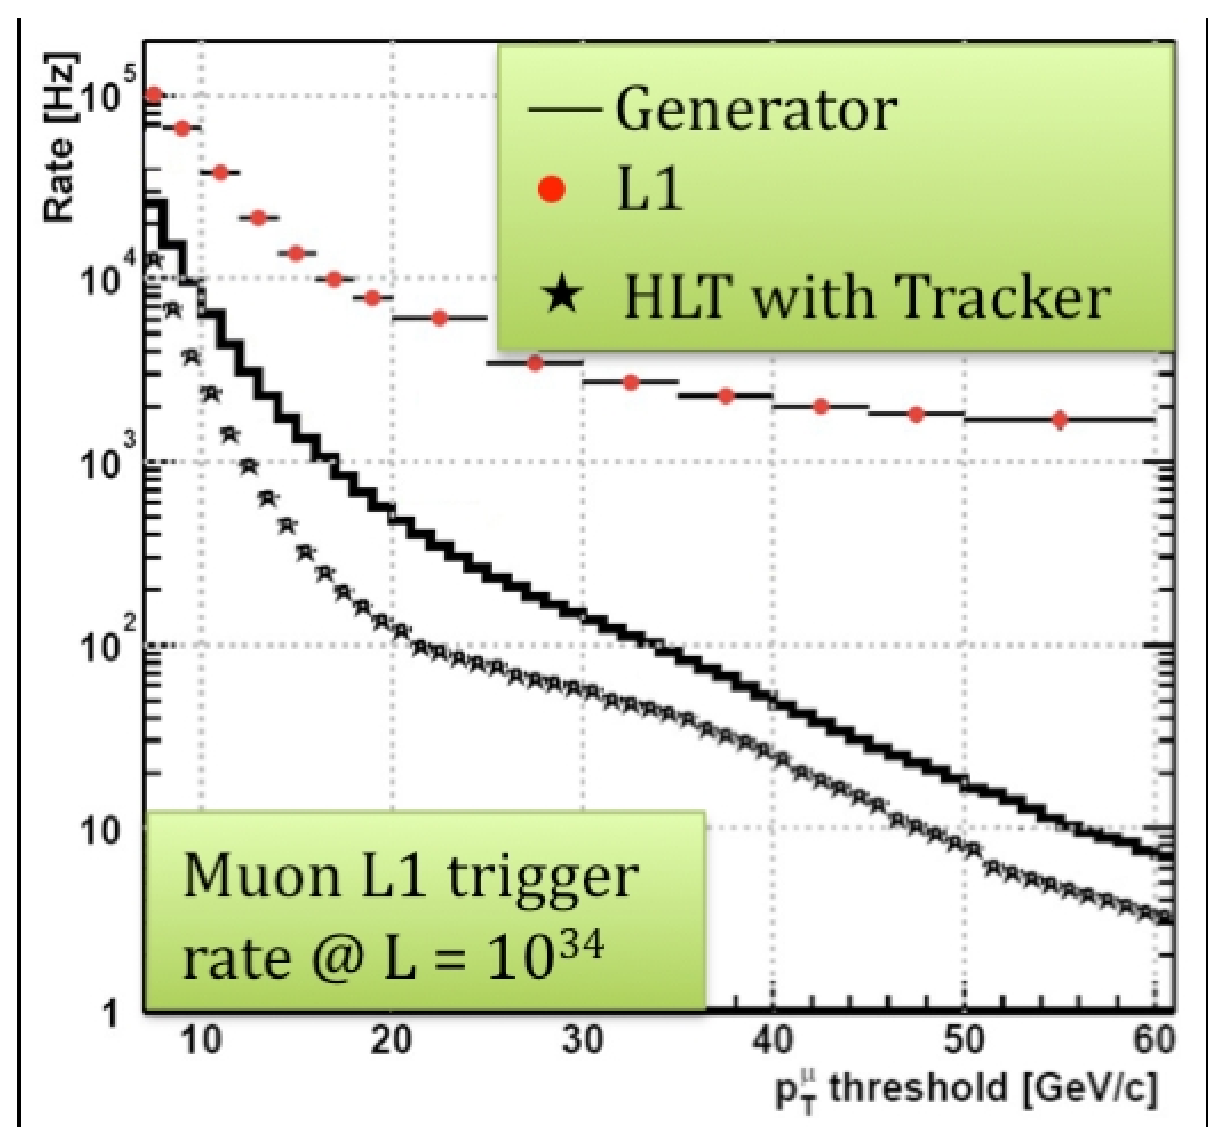
\includegraphics[width=0.99\textwidth]{Plots/CurrentTracker.eps}
\caption{Expected Level-1 single muon rate as a function of $p_{T}$ threshold for a luminosity of $10^{34}cm^{-2}s^{-1}$, in the present system.~\cite{bib:Abb-11}}
\label{fig:L1Rates}
\end{minipage}
\hfill
\begin{minipage}[t]{7.5cm}
\centering
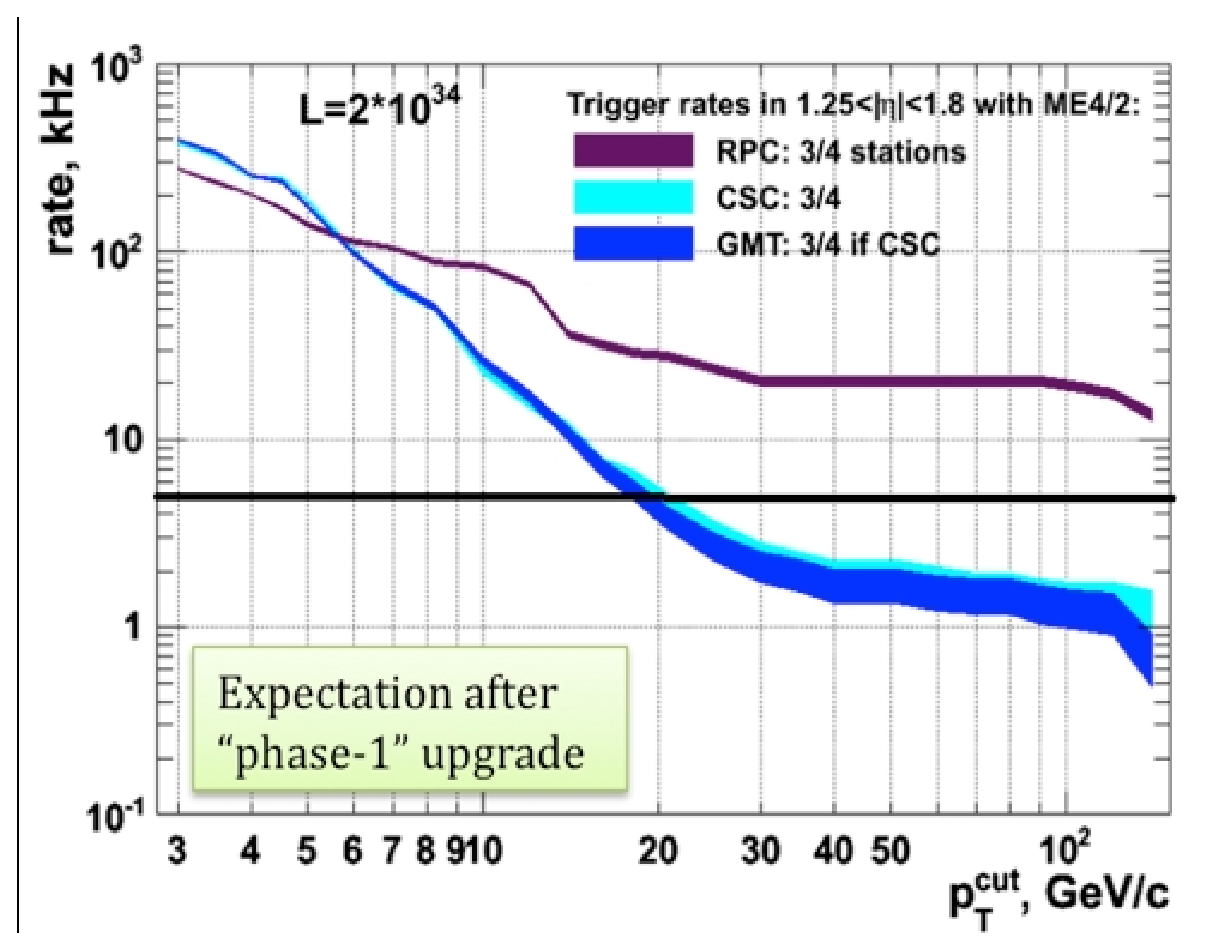
\includegraphics[width=0.99\textwidth]{Plots/21034_tracker.eps}
\caption{Expected threshold after phase 1 trigger upgrade, for a luminosity of $2\times 10^{34}cm^{-2}s^{-1}$.~\cite{bib:Abb-11}}
\label{fig:L1RatesPhase1}
\end{minipage}
\end{figure} 

\noindent One can also see on Fig.~\ref{fig:L1Rates} that fake proportion increases w.r.t. the $p_T$. This is due to the fact that L1 muon system uses coarse resolution information. Therefore high-$p_T$ tracks becomes compatible with straight lines at a certain point, and consequently the L1 muon rate reaches a plateau at high-$p_T$. At $10^{34}cm^{-2}s^{-1}$, this plateau lies at around $1~kHz$. Considering that overall L1 rate is $100~kHz$, the poor discrimination power at high-$p_T$ is not critical.

\noindent However, the plateau level is strongly depending on the instantaneous luminosity. Fig.~\ref{fig:L1RatesPhase1} shows its evolution, for the different muon subdetectors, at $2\times 10^{34}cm^{-2}s^{-1}$. For the RPC, the plateau lies at $20~kHz$, 20\% of the total L1 bandwidth. This is clearly not sustainable anymore. When going to HL-LHC luminosity, the other muons subdetectors also become problematic. In other words, muon indentification is not possible anymore. From there two solutions can be envisaged: increasing the L1 rate or including the tracking at L1. This note is dedicated to the second point.  

\noindent Our aim, in this document, is to procide a detailed description of such a system in the context of CMS. We tried to emulate the different stages of the hardware track fitting in order to estimate the feasibility/scaling of such a system with tracker geometry foreseen for CMS phase II upgrade. The simulation context, along with some estimation of the data rates that will be send to the trigger boards are presented in Section~{sec:FWork}. Pattern recognition is then described in Section~{sec:AM}. Finally, fitting stage is explained in Section~{sec:Fit}.

\clearpage

\section{CMS Track Trigger System Overview}

\subsection{Overview}

\begin{figure}[ht!]
\centering
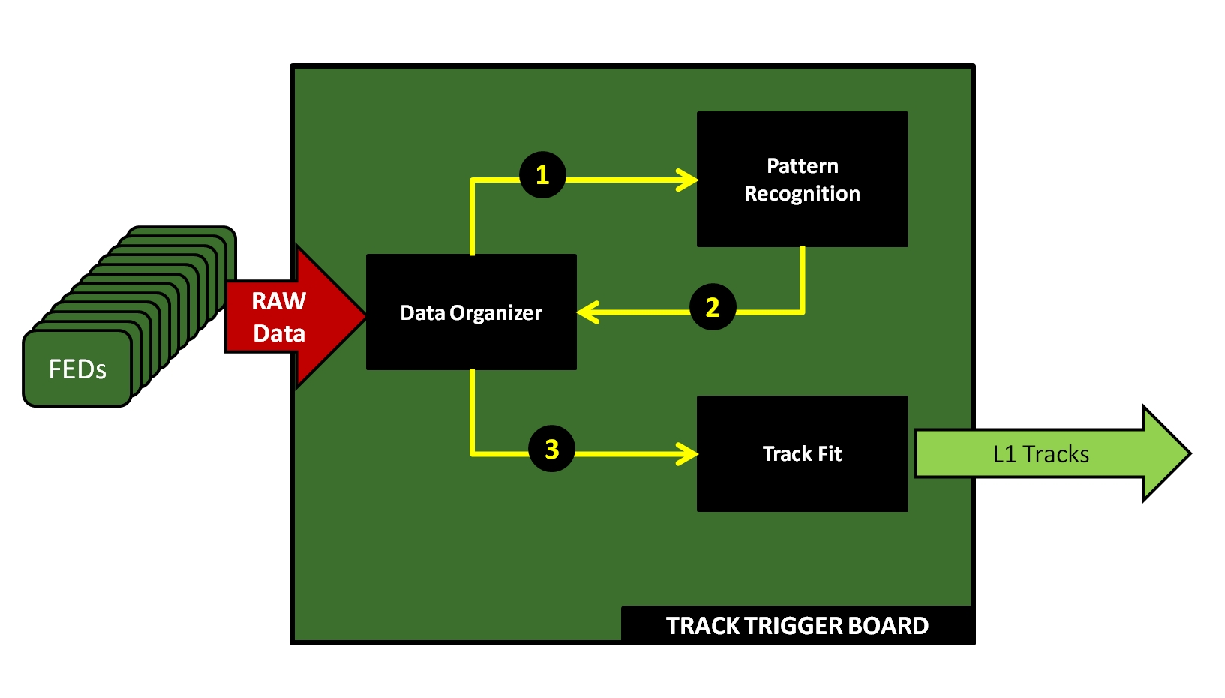
\includegraphics[width=0.5\columnwidth]{Plots/L1TTrigPrinciple.eps}
\caption{Hardware tracking principle}
\label{fig:L1TT_principle}
\end{figure}

\noindent Extracting track information is a two-stage process. First of all, you have to retrieve the hits belonging to the track: this is the pattern recognition. Then, you extract the track parameters (momentum, impact parameter,...) from the hits: this is the fit. Both steps are performed routinely in CMS, using very performant software algorithms. In order to pass to L1, tracking has to go hardware. Hardware-based tracking triggers were already developped in HEP experiments, in particular in the CDF experiment at Fermilab. Based on this system, the ATLAS experiment is planning to use a tracking trigger at the HLT after LHC long shutdown 2 in 2016. The working principle of these systems is sketched on Fig.~\ref{fig:L1TT_principle}. Tracker data is extracted by the FEDs and transmitted to the trigger board. Then, the data is handled by a data organization unit (DO), which extract the info necessary to the pattern recognition (PR), send it to the PR unit, and retrieve the matched patterns. The DO then sent the interesting hits to the track fit unit (TF), when the track parameters are estimated and sent to the L1 central trigger board.
\noindent In order to go at L1, one thus need the three following points: 

\begin{itemize}
\item A fast front-end readout system able to extract quickly all the data contained in the tracking detectors.
\item A system performing a fast pattern recognition.
\item A system performing a fast track fit.
\end{itemize}

\subsection{Interfaces}

\subsection{System architecture}

\subsection{Technical demonstrator concept}


\clearpage

\section{Vertical Slice Demonstrator System}

\subsection{System overview}



\clearpage

\section{Project organization}

\subsection{Institutions involved}

\subsection{Schedule and integration plan}

\subsection{Cost estimate}

\clearpage

\section{Conclusion}

\clearpage



%----------------------------------------
% Pour la bibliographie
%----------------------------------------

\newpage
\thispagestyle{empty}

\begin{thebibliography}{99}

%\bibitem{bib:Abb-11} D.~Abbaneo {\it for the CMS collaboration} - {\it "Upgrade of the CMS Tracker with tracking trigger"} - CMS CR -2011/284 (2011)

\bibitem{bib:Rist-89} M. Dell Orso, L. Ristori - {\it "VLSI Structure For Track Finding"} - Nucl.Instr. and Meth. A278 (1989), 436

\bibitem{bib:Ade-06} J. Adelman {\it et al.} - {\it "Real time secondary vertexting at CDF"} - Nucl.Instr. and Meth. A569 (2006), 111

\bibitem{bib:Ade-07} J. Adelman {\it et al.} - {\it "The Silicon Vertex Trigger upgrade at CDF"} - Nucl.Instr. and Meth. A572 (2007), 361

\bibitem{bib:Koh-87} T. Kohonen - {\it "Content-Addressable Memories"} - 2nd edition, New York, Springer- Verlag (1987)

\bibitem{bib:Pag-06} K. Pagiamtzis, A. Sheikholeslami - {\it "Content-Addressable Memory (CAM) Circuits and Archtectures: A Tutorial and Survey"} - IEEE Journal of Solid-State Circuits, Vol. 41, No. 3 (2006), 712


%\bibitem{bib:XML_wiki}\url{https://twiki.cern.ch/twiki/bin/view/CMSPublic/SWGuideGeomDevelopersGuide}

%\bibitem{bib:XML_oscar}\url{https://twiki.cern.ch/twiki/bin/view/CMSPublic/SWGuideOscarProducer}

%\bibitem{bib:G4SHits_cfi}\url{http://cmssw.cvs.cern.ch/cgi-bin/cmssw.cgi/CMSSW/SimG4Core/Application/python/g4SimHits_cfi.py?view=markup}

\bibitem{bib:Ann-06} A. Annovi {\it et al.} - {\it "A VLSI Processor for Fast Track Finding Based on Content Addressable Memories"} - IEEE Transactions on Nuclear Science, vol. 53, no. 4 (2006), 1

\bibitem{bib:Ann-09} A. Annovi {\it et al.} - {\it "The GigaFitter: A next generation track fitter to enhance online tracking performances at CDF"} - Nuclear Science Symposium Conference Record (NSS/MIC), 2009 IEEE (2009), 1143

\bibitem{bib:VIP-11}  - {\it "A New Concept of Vertically Integrated Pattern Recognition Associative Memory (VIPRAM)"} - FERMILAB-CONF-11-709-E, Proceedings of TIPP 2011 conference, Volume 37, 2012, Pages 1973

\bibitem{bib:VIP-12}  - {\it "Development of 3D Vertically Integrated Pattern Recognition Associative Memory (VIPRAM)"} - FERMILAB-TM-2493-CMS-E-PPD-TD

\bibitem{bib:FTK-10}  - {\it "FTK: A Hardware Track Finder for the ATLAS Trigger"} - Technical Proposal (2010)

%\bibitem{bib:Kar-91} V.~Karimaki - {\it "Effective circle fitting for particle trajectories"} - Nucl.Instr. and Meth. A305 (1991), 187

\end{thebibliography}
%----------------------------------------
% Annexes
%----------------------------------------
\newpage
\appendix

\section{Pattern recognition and track fitting approaches}

\subsection{Introduction to associative memory approach}

\noindent The CDF SVT-style associative memory approach, later adopted for FTK, consists of two sequential steps of increasing resolution.  In step 1, pattern recognition is carried out by a dedicated device called the Associative Memory (AM) which finds track candidates in coarse resolution roads.  When a road has stubs on all layers or all except one, step 2 is carried out in which the full resolution hits within the road are fit to determine the track helix parameters and a goodness of fit.  Tracks that pass a  2 cut are kept.  If there are hits in all layers and the  2 fails the cut but is not extremely large, the track is refit a number of times with the hit on one of the layers dropped each time.  This "majority recovery" allows for the loss of a single hit/stub due to detector inefficiency with a random hit picked up instead. 

\noindent Note that there has been more than a decade of experience in HEP with this approach from both CDF and Atlas, though all with silicon-based tracking trigger for Level 2 where trigger latency requirement is much more relaxed.  Therefore, one of the key issues for L1 implementation or demonstration will be the overall tracking trigger latency. Both the pattern recognition at the AM stage (hits delivery) and track fitting stage will have to be fast enough.


\subsubsection{From pattern recognition to track fitting}

\noindent The pattern recognition step is usually the most time consuming task, because one needs to test many combinations of hits to find those that potentially come from the same track and typically these tests are done sequentially (e.g. in software). The associative memory approach allows the testing of all hit combinations in parallel against a set of known patterns. To illustrate the concept of patterns in the associative memory approach, one can use an oversimplified case with a simple detector consisting of six detector layers, as shown in Fig.~\ref{fig:AM_principle_1}. A charged track crossing the detector would produce a set of hits (pattern). A finite set of distinct patterns can be generated this way using valid tracks for a given experiment, and such sets are often called the pattern bank. 

\begin{figure}[ht!]
\centering
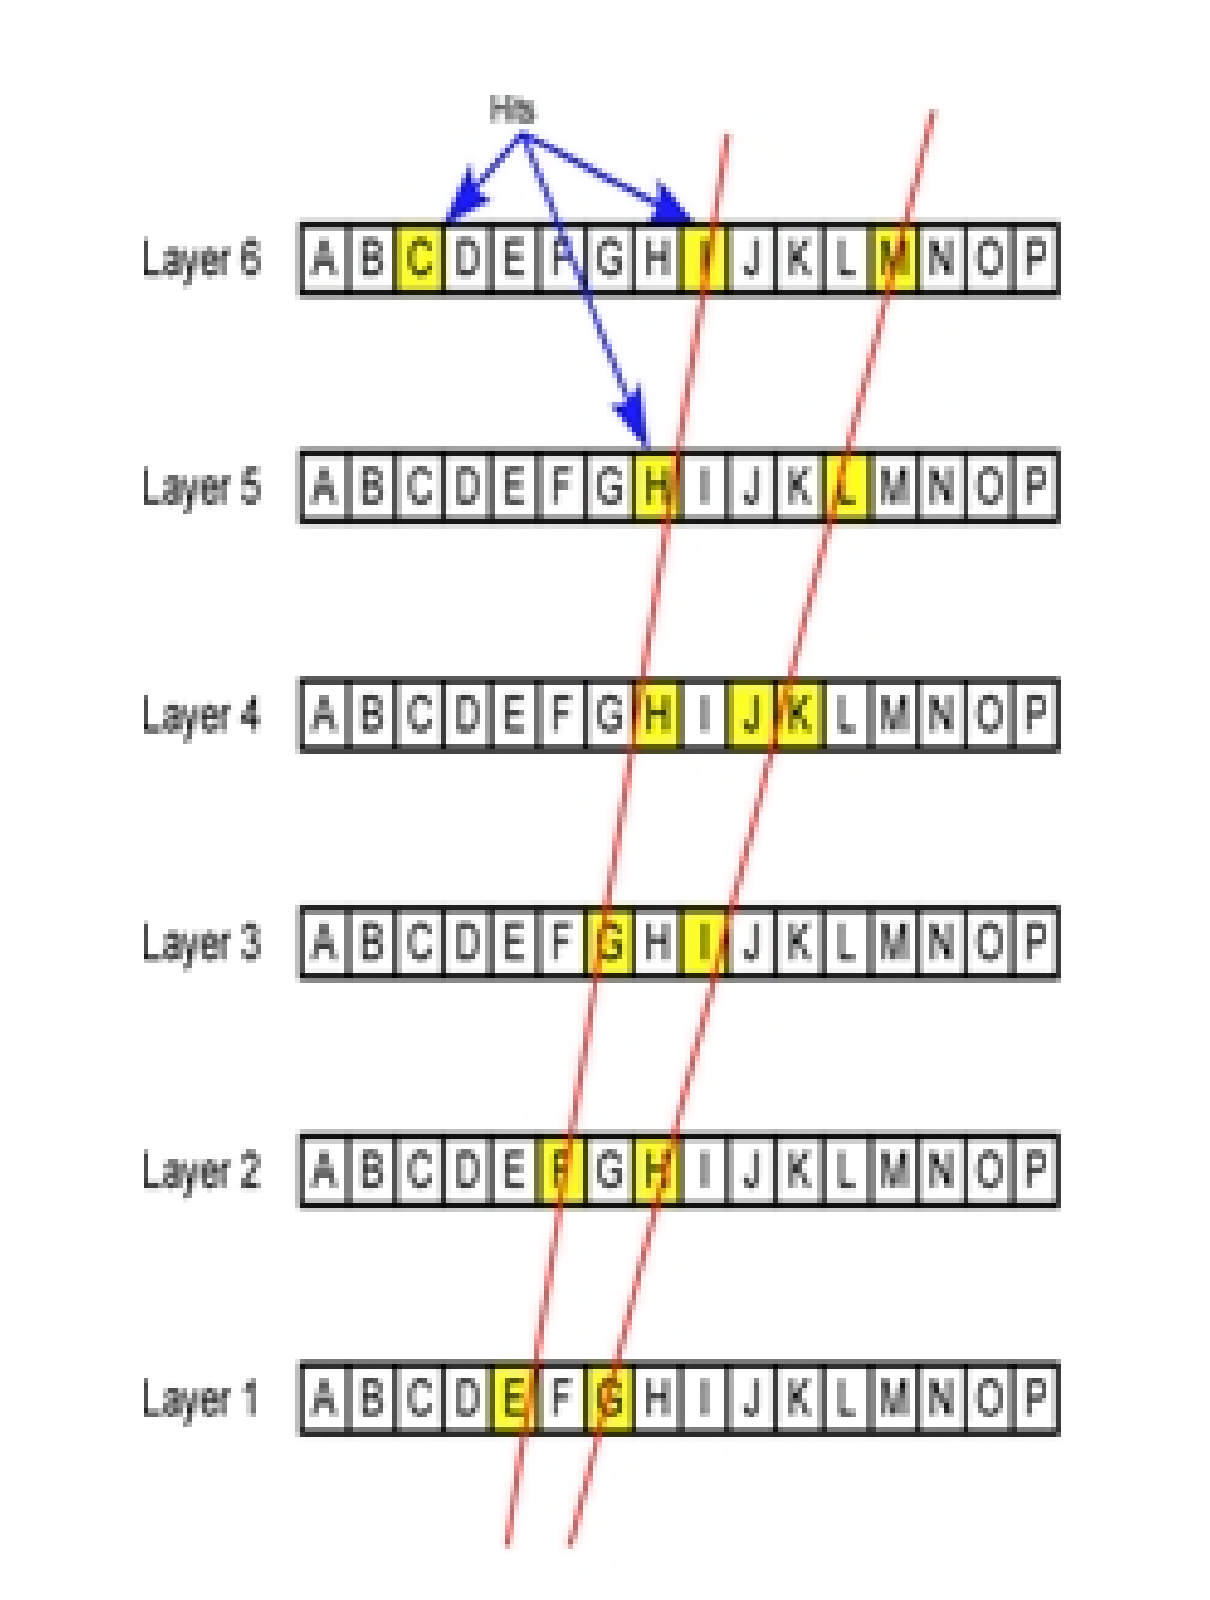
\includegraphics[width=0.4\columnwidth]{Plots/AM_pple2.eps}
\caption{Tracks in a tracking detector}
\label{fig:AM_principle_1}
\end{figure}

\noindent The Associative Memory (AM) architecture is based on Content Addressable Memory (CAM) cells~\cite{bib:Koh-87,bib:Pag-06} to efficiently identify track patterns (roads) at high speed using coarse-resolution 'hits' recorded in the tracking detector. A block diagram~\cite{bib:Rist-89} of the Associative Memory architecture is shown in Fig. 2 (for a case with four detector layers).  Each pattern (shown as a cell) is composed of four hit coordinates each of which is stored in the CAM word for a given layer, and only four patterns (cell 0 to 3) are shown in Fig.~\ref{fig:AM_principle_2}. 

\begin{figure}[ht!]
\centering
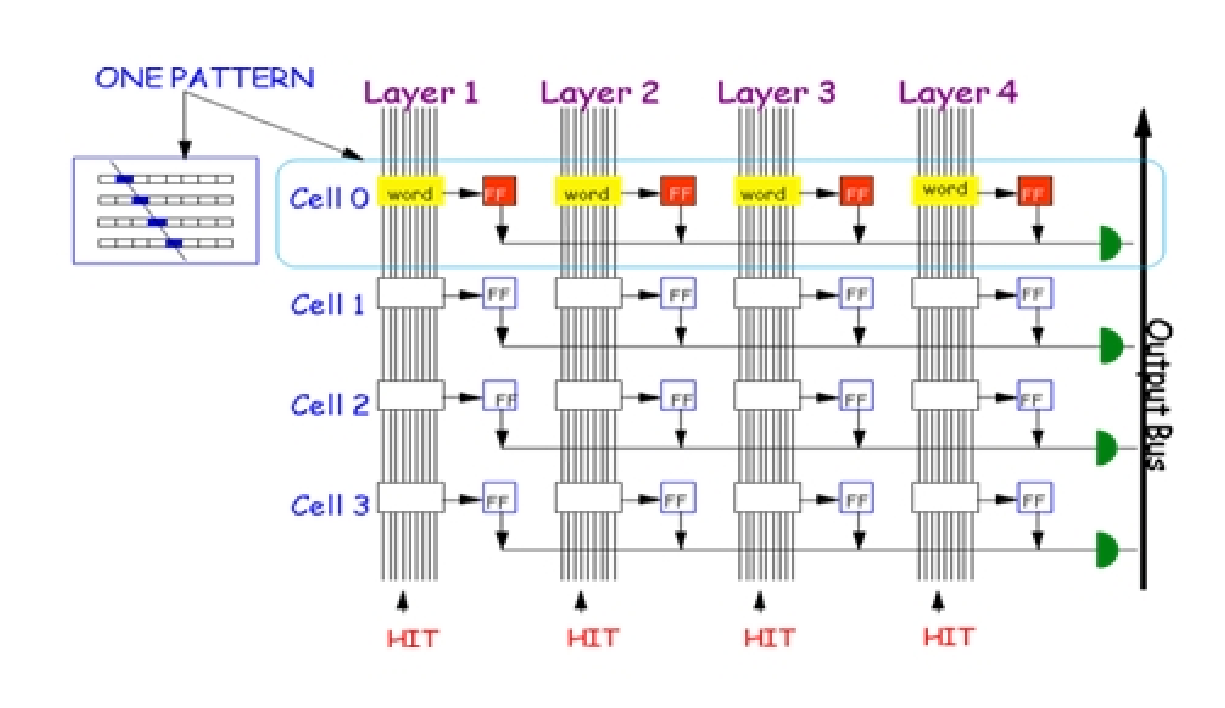
\includegraphics[width=0.9\columnwidth]{Plots/AM_pple.eps}
\caption{A block diagram on an associative memory chip. The CAM cells are shown as white (or yellow) boxes. The majority/glue logic is shown to the right as semi-circles.}
\label{fig:AM_principle_2}
\end{figure}

\noindent An incoming hit from a given detector layer is transmitted to the corresponding layer and the hit coordinate is compared against the stored words for all patterns in parallel for that layer. Any match to each incoming hit will be latched for that layer an
d for that pattern until reset (to rearm for next event). This process is repeated for all the incoming hits for each detector layer as the hits arrive one after the other. As soon as all hits from the same event are received, the hit matching stage is done and all latched matches for each pattern (or cell) will be fed into a majority logic stage where a fired road will be found if the number of matched layers reaches a programmable threshold. 
 

\noindent Associative Memory is sometimes called PRAM, Pattern Recognition Associative Memory. The AM method solves the combinatorial challenge inherent to the pattern recognition by exploiting massive parallelism of associative memories that can compare tracking detector hits to a set of pre-calculated patterns simultaneously. The found patterns or "fired roads" are then processed using fast FPGAs to perform track fitting with full detector resolution using all combinations of the "hits of interest" from the fired roads. Because each pattern or road is narrow enough, the usual helical fit can be replaced by a simple linear calculation. The track fitting stage for each matched pattern is much simplified and can be very fast~\cite{bib:Ann-09}.

\subsection{Sector, superstrip, and pattern banks}

\noindent The pattern generation procedure starts by identifying first the sectors, which consists of one silicon module in each detector/logical layer. The list of sectors is determined with a training procedure that uses a large number of single muon (negative and positive) events, to cover all possible combinations of modules compatible with tracks coming from a region around the nominal beam spot position. The concept of sector is important because it is the region in which the linear track fit with one set of constants is performed (see later track fitting stage).

\noindent Each pattern is made of one superstrip per layer. A superstrip is a group of strips/pixels, and is therefore heavily constrained by the detector itself. Once the superstrip definition has been set, its position information is coded in a N-bits word: the superstrip address. It is important to realize that the AM-based pattern recognition is using these addresses, and is therefore independent from the detector geometry. As the addresses are transmitted to the AM independently for each layer, layer number doesn't have to be in the address word. 

\begin{figure}[ht!]
\centering
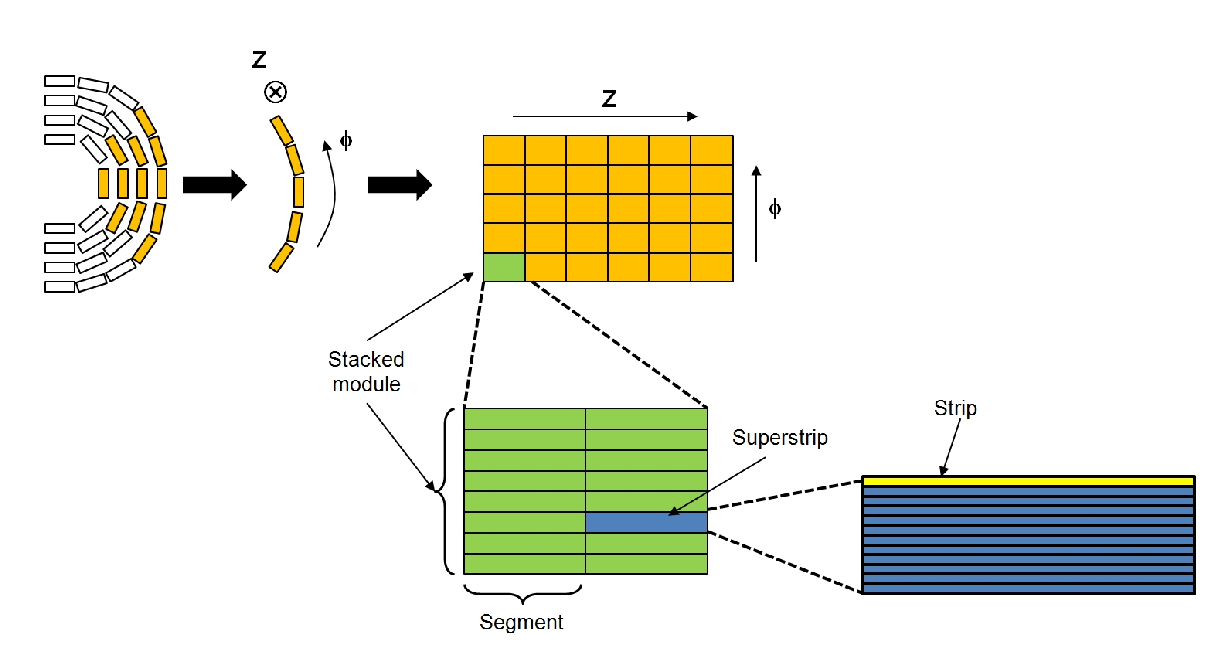
\includegraphics[width=0.8\columnwidth]{Plots/SStripDef.eps}
\caption{Geometric definition of a superstrip (barrel example).}
\label{fig:Det_to_SS}
\end{figure}
\begin{figure}[ht!]
\centering
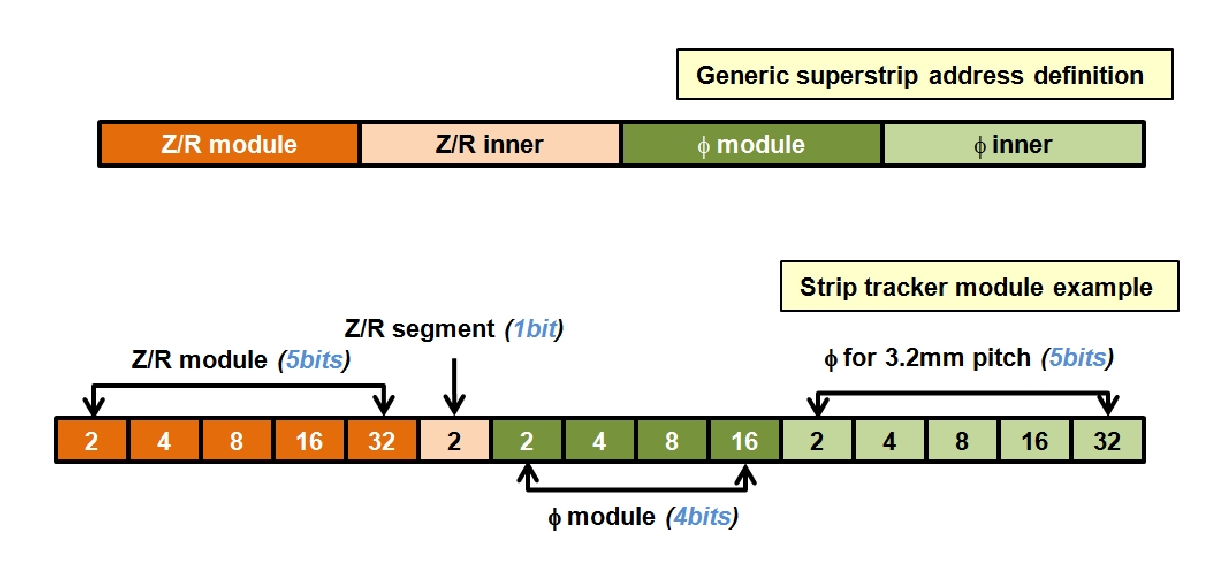
\includegraphics[width=0.6\columnwidth]{Plots/SSaddress.eps}
\caption{Address definition of a superstrip.}
\label{fig:SS_def}
\end{figure}

\noindent In order to understand the address definition, Fig.~\ref{fig:Det_to_SS} shows how a superstrip is defined in the barrel part of the tracker. Figure~\ref{fig:SS_def} shows the address definition of a superstrip. The number of bits necessary reflects the superstrip granularity and is constrained by the maximal word size acceptable by the AM chip (default is 15 bits). A first set of bits provides the module number along the corresponding coordinate: 5 bits for Z (one could have up to 24 modules in Z in one sector) and 4 for ? (up to 11 modules per sector in the outermost layer). Then, for each coordinates, a second series of bits provide the superstrip position within the module. Fig. 6 shows a tracker strip module (in green), divided into 2 segments in Z and 1024 strip in ?. Therefore in order to describe all the position, one would need only 1 bit for Z, and 10 bits for ?. In practice, a certain number of strips are grouped to form the superstrip, in our case 32, thus leading to 5 in the address. For the endcap the coding is the same, with z being replaced by r (equivalence is made between disks and layers, ladders and rings). 



\clearpage

\section{Simulation tool development}

\subsection{The importance of simulation tools}

\noindent AM-based track reconstruction is a complex procedure requiring a significant amount of preparation. This preparation is done via a dedicated simulation framework. This framework should provide the following features:

\begin{itemize}
\item A modelization of the new tracker geometry implemented in the CMS software framework (CMSSW)
\item A tool for optimization of the trigger tower definition
\item A tool performing the pattern bank generation
\item A program emulating the AM-based pattern recognition procedure
\item A track fitting procedure compatible with an FPGA implementation  
\end{itemize}

\noindent This section is providing a description of these steps for the CMS L1 trigger application. 

\subsection{Tracker geometry and trigger tower definition}

\noindent Here we place a description of the TkLayout tool

\subsection{Pattern bank generation}

\noindent Bank generation is done using a standalone C++ code developed on purpose. The basic procedure is sketched on Fig.~\ref{fig:BkGen}. In order to produce a bank, two inputs are needed: a clean and large sample of particle gun track (traditionally muons), and a definition of the trigger towers. Both inputs are easily obtained using the tools described in the previous part. 

\begin{figure}[ht!]
\centering
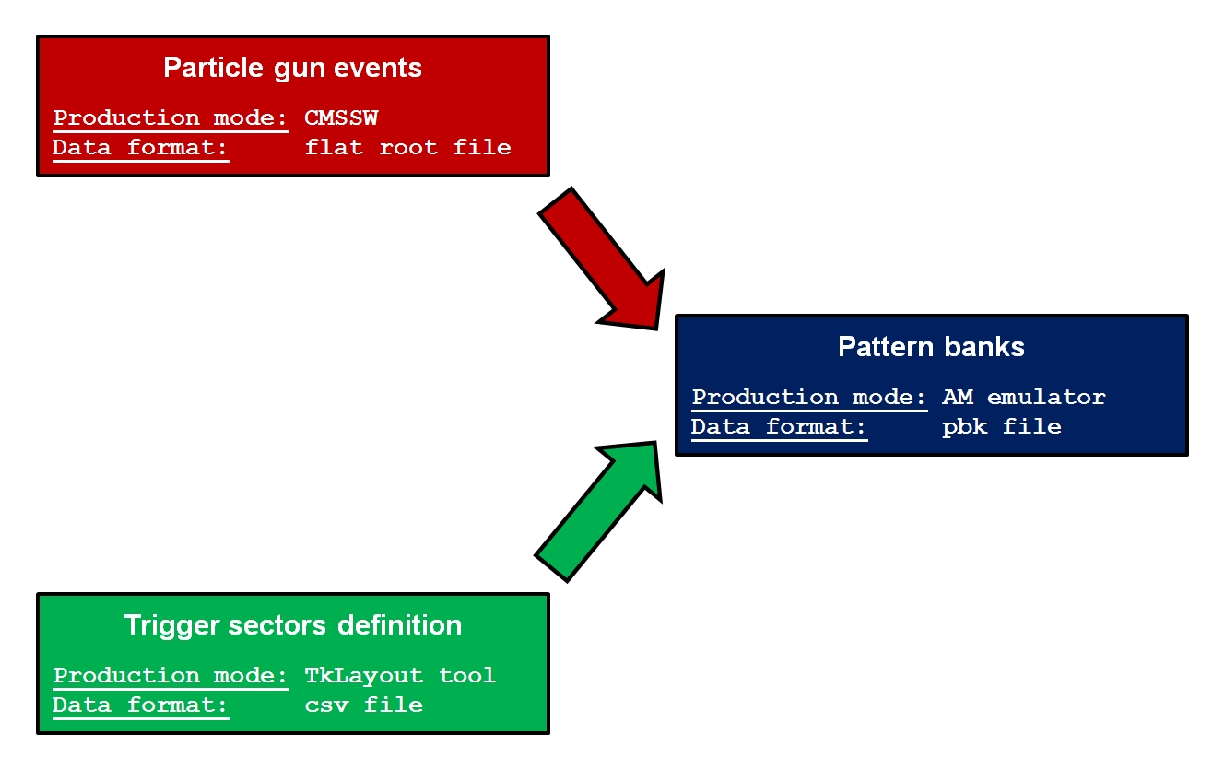
\includegraphics[width=0.6\columnwidth]{Plots/BankGen.eps}
\caption{Pattern bank generation principle}
\label{fig:BkGen}
\end{figure}

\noindent Based on these inputs, the code is able to generate a pattern bank for a given trigger tower. Bank parameters can be set in the configuration file of the bank generation job. In particular, AM chip specific mechanism such as don't care (DC) bits have been implemented. The bank generation data-flow is summarized on Fig.~\ref{fig:BkGenDet}.

\begin{figure}[ht!]
\centering
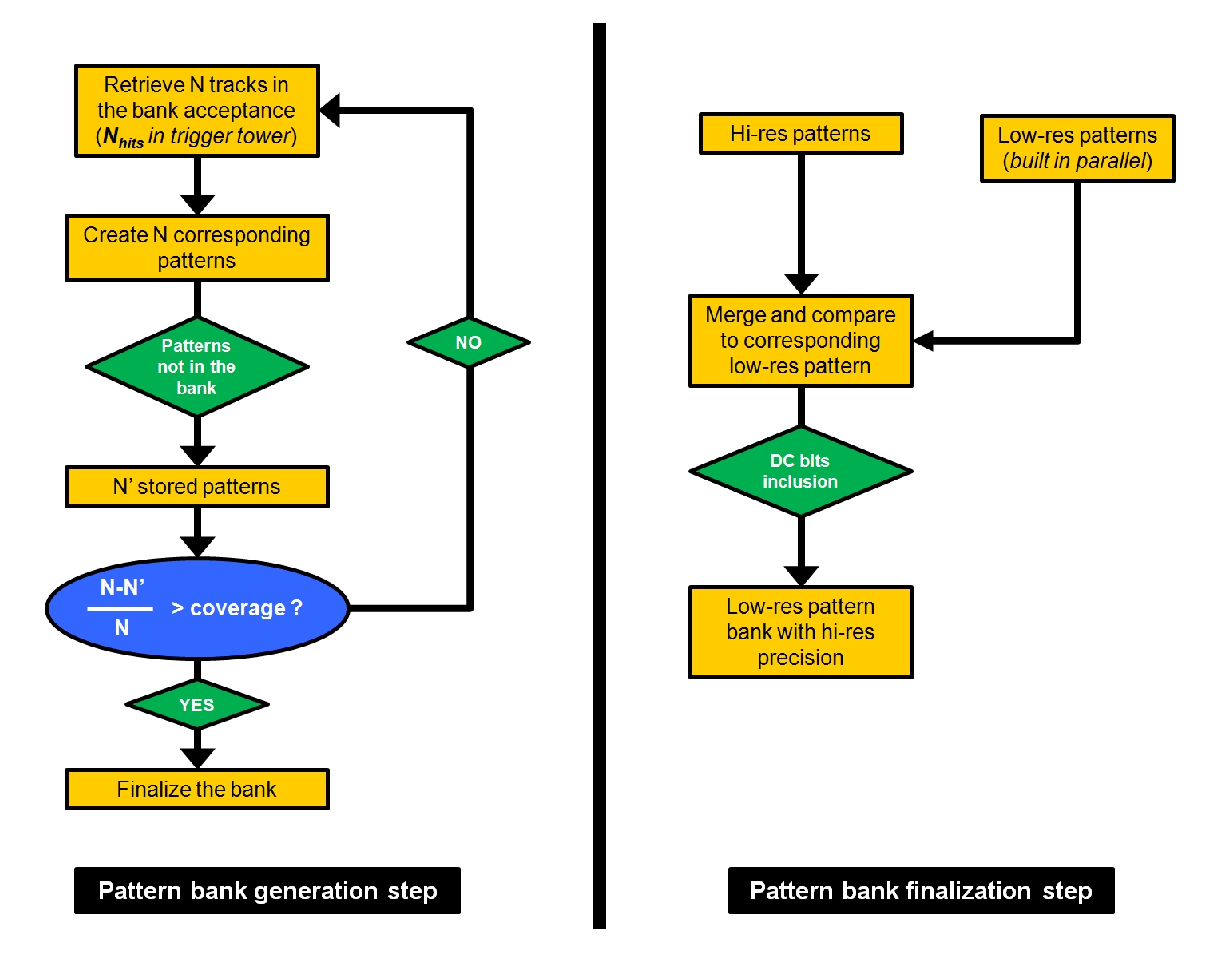
\includegraphics[width=0.6\columnwidth]{Plots/BankGenDetail.eps}
\caption{Pattern bank generation workflow: from track sample to pattern bank}
\label{fig:BkGen}
\end{figure}

\noindent The flow can be divided into two steps: the bank production and the bank finalization. As shown on the left diagram, the bank production is done iteratively. An iteration starts with the collection of tracks satisfying the pattern bank acceptance requirements in the input data sample. This acceptance requirement is defined by the parameter $N_{hits}$, which corresponds to the number of different layer/disks in which the particle has induced a stub in the trigger tower considered. This number should not be confused with the total number of stubs induced by the particle.

\noindent A track will be used to produce a pattern only if $N_{hits}+1$ is larger of equal to the pattern size (we accept the possibility of having one missing hit on the track). In this case, a pattern corresponding to the track is created and stored in the bank if not already in. Iteration ends when a sufficient number of tracks have been collected. At this point, the proportion of tracks collected which were already in the bank is computed. If this proportion is larger than the coverage initially requires, the iteration stage stops.

\noindent Once the required coverage has been reached, the bank is finalized. The procedure is described in the right part of Fig.~\ref{fig:BkGenDet}. At this point two banks have been built. Indeed, every pattern added to the bank produced at the iteration process is linked to a mother pattern of lower resolution. The resolution of this mother pattern is direclty related to the number of DC bits added, the width of the low-res roads is indeed $2^{N_{DC}}$ larger than for the initially built roads. For example, if one requires 2 DC bits, and built pattern with a superstrip size of 32 strips, the width of the low resolution patterns will be 128 strips. 

\noindent At the end of the iterative procedure, each low-res patterns is linked to a set of hi-res patterns. Before storing the low-res pattern in the banks, hi-res patterns belonging to it are merged. The merging result is then compared to the low-res pattern, and the hi-res granularity is kept whenever possible. On the other hand, if all the super-strips are used in a given layer, corresponding DC bits are applied.

\noindent The main advantage of the DC bits procedure is to get high-resolution precision for the price of a low resolution bank. 


\subsection{Pattern recognition}

\subsubsection{Software principle}

\subsubsection{Estimation of the pattern recognition efficiencies and fake rates}


\noindent The generation of the patterns bank is done using a Monte Carlo samples of particle gun $\mu^{\pm}$ produced within the following phase space:
\begin{itemize}
\item $0 < \eta_0 < 2.2$.
\item $1.95GeV/c < p_{T_0} < 100GeV/c$, generated randomly in $1/p_T$.
\item $-15cm < z_0 < 15cm$.
 \item $-1mm < d_0 < 1mm$.
\end{itemize}  

\noindent The direction of the transverse impulsion ($\phi_0$) is chosen such that the generated particles cover the sector we are interested in. The generation procedure is iterative and is using only tracks containing exactly one stub per layer/disk. At iteration $n$, a set of $N$ such tracks is collected. Then one computes the PR efficiency for those tracks using the pattern bank obtained at the end of iteration $n-1$. If the efficiency is larger than a given threshold (called the coverage), the procedure stops. Otherwise, the new patterns formed with those tracks are added to the bank and iteration $n+1$ is done. 

\noindent At the beginning of the first iteration, the bank being empty, every particle will lead to a new pattern insertion. Then, as the bank is being populated, the efficiency growth will become slower.

\subsubsection{Bank efficiency definition}

\noindent Let's denote $N$ the number of tracks you want to reconstruct in a given event, ie the tracks which are within the L1 track trigger requirements. Then, we denote $N^{matched}$ the number of tracks which are contained into at least one pattern. The PR efficiency $\epsilon$ can thus be defined as: 
\begin{equation}
\epsilon = \frac{N^{matched}}{N}
\end{equation} 

\noindent Then, we note $N_{pattern}$ the total number of patterns activated in the event and $N^{matching}_{pattern}$ the number of patterns containing one of the tracks we are looking for. From there one could define the fake rate $\rho$:
\begin{equation}
\rho = 1 - \frac{N^{matching}_{pattern}}{N_{pattern}}
\end{equation} 

\noindent Another important figure is the redundancy $r$. It corresponds to the average number of patterns activated by a good track. 

\noindent Last but not least, one should keep in mind that the PR goal is to provide low-sized hit sets for the track fitting (TF) stage in order to reduce the combinatorics, and consequently the TF time budget. The proportion of good hits per pattern, noted $\epsilon_{hits}$ is therefore a very important parameter:
\begin{equation}
\epsilon_{hits} = \frac{1}{N_{pattern}}\sum_{N_{pattern}}\frac{N_{hits}^{good}}{N_{hits}}
\end{equation} 

\noindent The ideal pattern bank is the one for which:  
\begin{enumerate}
\item $\epsilon = 1$.
\item $\rho = 0$.
\item $r = 1$.
\item $\epsilon_{hits} = 1$. 
\end{enumerate}  

\noindent This ideal bank exists, this is the one for which each possible track in the detector corresponds to one pattern. However, the size of such bank is clearly prohibitive. On the other side, one could imagine the simplest bank with 1 single pattern defined by the whole detector. Such a bank will have $\epsilon=1$, $\rho = 0$ and $r = 1$, but $\epsilon_{hits}$ will be close to 0. Such a solution would be highly inefficient, as TF would be impossible to process. Therefore the optimal solution lies in between, and one realizes that a parameter will be very important: the size of the patterns. The patterns will have to be sufficiently small in order to get a reasonable $\epsilon_{hits}$, but also sufficiently large in order get a reasonable pattern bank size. 


\subsection{Further developments and improvements}


\clearpage

\section{Track Trigger Performance Requirements}

\subsection{Tracking performance}

\subsection{Performance on trigger objects}

\subsection{Selected physics cases}

\clearpage


\end{document}
